\documentclass[16pt]{beamer}

\usepackage[french]{babel}
\usepackage[T1]{fontenc}
\usepackage[utf8]{inputenc}
\usepackage{graphics}
\usepackage{graphicx}
\DeclareMathSizes{16}{36}{22}{18}
\hypersetup{pdfpagemode=FullScreen}
\usetheme{Szeged}
\usecolortheme{beaver}
\setbeamertemplate{itemize item}{\color{red}$\blacktriangleright$}
\setbeamertemplate{itemize subitem}{\color{red}$\blacktriangleright$}
\setbeamercolor{local structure}{fg=red}
% \usefonttheme{serif}
\title{Algorithme génétique: application au problème du voyageur de commerce}
\author{Mathieu Mandret}
\institute{IUT Paul Sabatier}

\begin{document}
% Page de titre
\begin{frame}
  \maketitle
  \centering
  
\includegraphics[scale=0.05]{logo_IUT.png}
\end{frame}

% Sommaire
\begin{frame}
  \frametitle{Plan}
  \tableofcontents
\end{frame}

% Problème du voyageur de commerce
\section{Le problème du voyageur de commerce}
\begin{frame}
  \frametitle{Le problème du voyageur de commerce}
  \begin{itemize}
    \item $n$ villes.
    \item Les parcourir une fois.
    \item Revenir au point de départ.
    \item Chemin le plus court?
  \end{itemize}
\end{frame}

\begin{frame}
  \frametitle{Le problème du voyageur de commerce}
  \begin{center}
    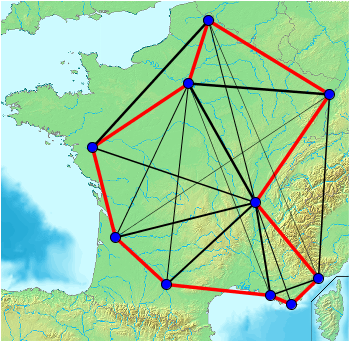
\includegraphics[scale=0.7]{Carte_france_10_villes.png}
  \end{center}
\end{frame}

\begin{frame}
  \frametitle{Approche déterministe}
  Permutations de $n$ éléments:
  \[
  \begin{array}{r c l}
  n &=& 10 \\
  n! &=& 3 628 880
  \end{array}
  \]
\end{frame}

\begin{frame}
  \frametitle{Approche déterministe}
  Permutations de $n$ éléments:
  \[
  \begin{array}{r c l}
  n &=& 30 \\
  n! &\simeq& 2.65 \times 10^{32}
  \end{array}
  \]
\end{frame}

\begin{frame}
  \frametitle{Approche déterministe}
  \[
  \begin{array}{r c l}
  1 \text{ permutation} &=& 10^{-9}s \\ \pause{}
  2.65 \times 10^{32} \text{ permutations} &=& 2.65 \times 10^{32} \times 10^{-9}s
  \end{array}
  \]
\end{frame}

\begin{frame}
  \frametitle{Approche déterministe}
  \[
  2.65 \times 10^{32} \text{ permutations} = 2.65 \times 10^{23}s
  \]
\end{frame}

\begin{frame}
  \frametitle{Approche déterministe}
  \[
  \frac{2.65 \times 10^{23}}{3.154 \times 10^{7}} \text{ années}
  \]

\end{frame}

\begin{frame}
  \frametitle{Approche déterministe}
  \[
  8.4 \times 10^{15} \text{ années}
  \]
\end{frame}

\section{Algorithmes génétiques}

\begin{frame}
  \frametitle{Principe général}
  \begin{itemize}
    \item Solution approchée
    \item Inspiré de la théorie de l'évolution
    \item Sélection naturelle
  \end{itemize}
\end{frame}

\begin{frame}
  \frametitle{Déroulement}
  \begin{columns}
    \column{0.6\linewidth}
        \centering
            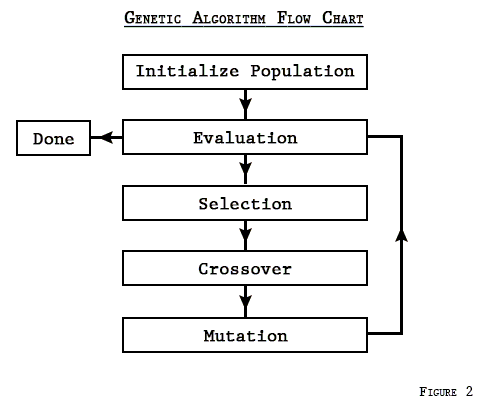
\includegraphics[scale=0.4]{GA.png}
    \column{0.4\linewidth}
        \begin{enumerate}
            \item Générer population \pause{}
            \item Calculer toutes les fitness \pause{}
            \item Sélectionner les parents \pause{}
            \item Les croiser \pause{}
            \item Faire muter les fils
        \end{enumerate}
  \end{columns}
\end{frame}

\begin{frame}
  \frametitle{Déroulement}
  Boucle $\rightarrow$ condition d'arrêt:
  \begin{itemize}
    \item Nombre de générations
    \item Fitness cible 
  \end{itemize}
\end{frame}

\section{Application au problème du voyageur du commerce}
\begin{frame}
  \frametitle{Application au problème du voyageur du commerce}
  \begin{block}{}
\[
  \begin{array}{r c l}
    \text{Individu } &\rightarrow& \text{ Chemin} \\
    \text{Population } &\rightarrow& \text{ Ensemble de chemins} \\
    \text{Fitness } &\rightarrow& \text{ Longueur du chemin} 
   \end{array}{}
\]
\end{block}
\end{frame}

\begin{frame}[fragile]
\frametitle{Architecture orientée objet}
\framesubtitle{\textbf{Ville}}
Coordonnées (X,Y) \\
Distance par rapport à une autre ville
\end{frame}

\begin{frame}
  \frametitle{Ville}
  \framesubtitle{Distance entre 2 villes}
  \begin{center}
  \[
    ||\overrightarrow{AB}|| = \sqrt{(x_b - x_a)^2 + (y_b - y_a)^2} \\
  \pause{}
  \text{math.hypot}(x_b - x_a, y_a -  y_b)
  \]
  \end{center}
\end{frame}

\begin{frame}
  \frametitle{Architecture orientée objet}
  \framesubtitle{\textbf{Chemin}}
  \begin{itemize}
    \item Liste ordonnée de ville
    \item Calcul de la fitness
  \end{itemize}
\end{frame}

\begin{frame}
  \frametitle{Chemin}
  \framesubtitle{Fitness d'un chemin}
  \[
    \sum_{i}^{n-1} ||\overrightarrow{V_{i}V_{i+1}}||
  \]
\end{frame}

\begin{frame}
  \frametitle{Chemin}
  \framesubtitle{Partially Matched Crossover}
    \begin{enumerate}
      \item Prendre $x$ villes du parent 1
      \item Les mettre dans les positions correspondante dans le fils
      \item Remplir le reste avec des villes du parent 2
    \end{enumerate}
\end{frame}

\begin{frame}
  \frametitle{Chemin}
  \framesubtitle{Partially Matched Crossover}
    \begin{enumerate}
      \item Prendre $x$ villes du parent 1
      \item Les mettre dans les positions correspondante dans le fils
      \item Remplir le reste avec des villes du parent 2
    \end{enumerate}
\end{frame}

\begin{frame}
  \frametitle{Chemin}
  \framesubtitle{Partially Matched Crossover}
  \begin{figure}
    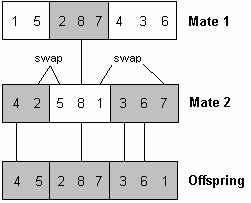
\includegraphics[scale=0.9]{pmx.png}
    \end{figure}
\end{frame}

\begin{frame}
  \frametitle{Architecture orientée objet}
  \framesubtitle{\textbf{Population}}
  \begin{itemize}
    \item Initialisation
    \item Évolution
      \begin{itemize}
        \item Sélection
        \item Mutation
      \end{itemize}
    \item Condition d'arrêt
  \end{itemize}
\end{frame}

\begin{frame}
  \frametitle{Population}
  \framesubtitle{Initialisation}
  Chemin uniques $\rightarrow$ Diversité \\
  Opérateur \emph{not in}
\end{frame}

\begin{frame}
  \frametitle{Population}
  \framesubtitle{Sélection}
  Tournoi
  \begin{enumerate}
    \item Prendre $x$ individus au hasard
    \item Sélectionner le meilleur 
  \end{enumerate}
\end{frame}

\begin{frame}
  \frametitle{Population}
  \framesubtitle{Sélection}
  \begin{figure}
    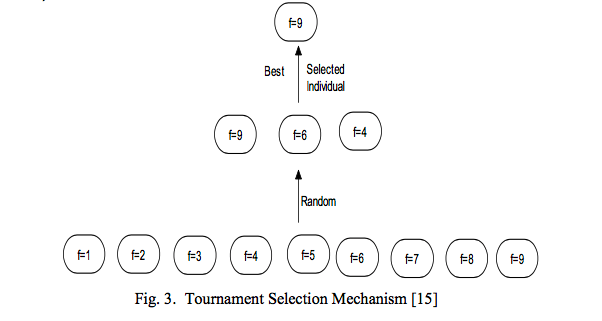
\includegraphics[scale=0.4]{tournament.png}
  \end{figure}
\end{frame}

\begin{frame}
  \frametitle{Population}
  \framesubtitle{Sélection}
  \centering
  Roulette \pause{}
  \begin{figure}
    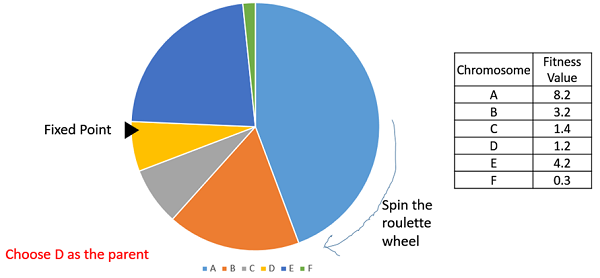
\includegraphics[scale=0.6]{roulette.jpg}
  \end{figure}
\end{frame}

\begin{frame}
  \frametitle{Population}
  \framesubtitle{Sélection}
  \centering
  Roulette
  \begin{enumerate}
    \item Sommer toutes les fitness
    \item Prendre un nombre aléatoire en 0 et la somme
    \item Tant que ce nombre n'est pas 0 ou moins 
    \item Se positionner un chemin
    \item Soustraire au nombre la fitness du chemin courant
    \item Passer au chemin suivant
  \end{enumerate}
\end{frame}

\begin{frame}
  \frametitle{Population}
  \framesubtitle{Sélection: Complexité}
  Recalculer la longueur de tous les chemins \\
  En faire la somme \\ \pause{}
  \textbf{Utiliser un cache}
\end{frame}

\begin{frame}[fragile]
  \frametitle{Population}
  \framesubtitle{Sélection: Cache}
  \[
    [\text{Chemin}] \Rightarrow \text{fitness} \pause{}
  \]
  \[
   \textbf{Si } \text{chemin} \in \text{clés} \text{ récupérer } \textbf{sinon} \text{ calculer}
  \]
\end{frame}

\begin{frame}
  \frametitle{Population}
  \framesubtitle{Mutation}
  \begin{enumerate}
    \item Swap
    \item Scramble
  \end{enumerate}
\end{frame}

\begin{frame}
  \frametitle{Population}
  \framesubtitle{Mutation}
  \begin{enumerate}
    \item Swap $\rightarrow$ échanger 2 villes
    \item Scramble $\rightarrow$ mélanger les villes entre 2 bornes
  \end{enumerate}
\end{frame}

\section{Résultats}
\begin{frame}
  \frametitle{Mesurer l'efficacité}
  \framesubtitle{Pourcentage d'amélioration}
  \centering
  Mesure à quel point les chemins sont devenus meilleurs sur $n$ générations \pause{}
  \[
    \frac{\text{Meilleure fitness}_1}{\text{Meilleure fitness}_n} \times 100
  \]
\end{frame}

\begin{frame}
  \frametitle{Mesurer l'efficacité}
  \framesubtitle{Pourcentage d'amélioration}
  \begin{figure}
    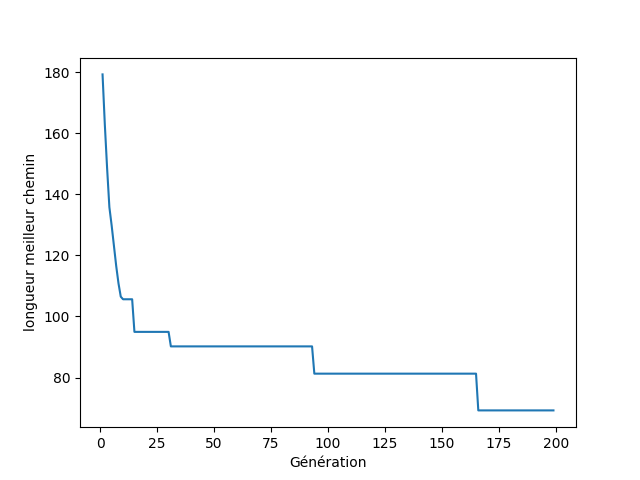
\includegraphics[scale=0.5]{evol.png}
  \end{figure}
\end{frame}

\begin{frame}
  \begin{figure}
  \frametitle{Mesurer l'efficacité}
  \framesubtitle{Pourcentage d'amélioration}
    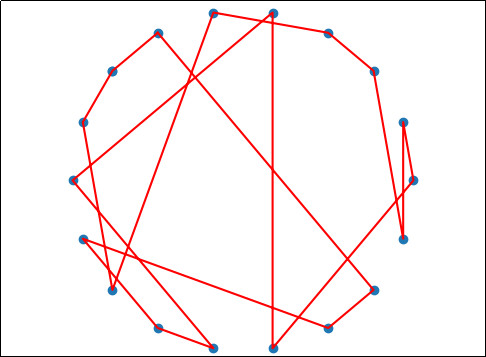
\includegraphics[width=0.5\textwidth]{gen1.png}
    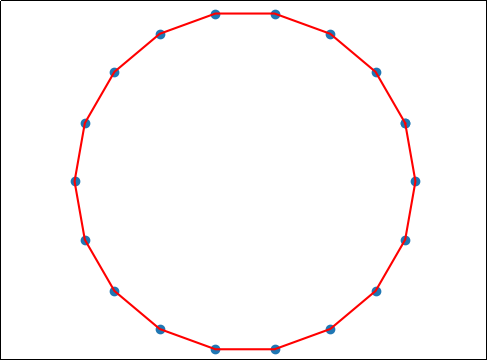
\includegraphics[width=0.5\textwidth]{gen200.png}
  \end{figure}
\end{frame}

\section{Conclusion}

\begin{frame}
  \frametitle{Conclusion}
  \pause{}
  Difficultés: Crossover, et roulette.
\end{frame}

\end{document}
